% WU-5 figures — generated by scripts/build_faithfulness_axis.py (regenerate; do not edit numbers)
\begin{figure}[t]
  \centering
  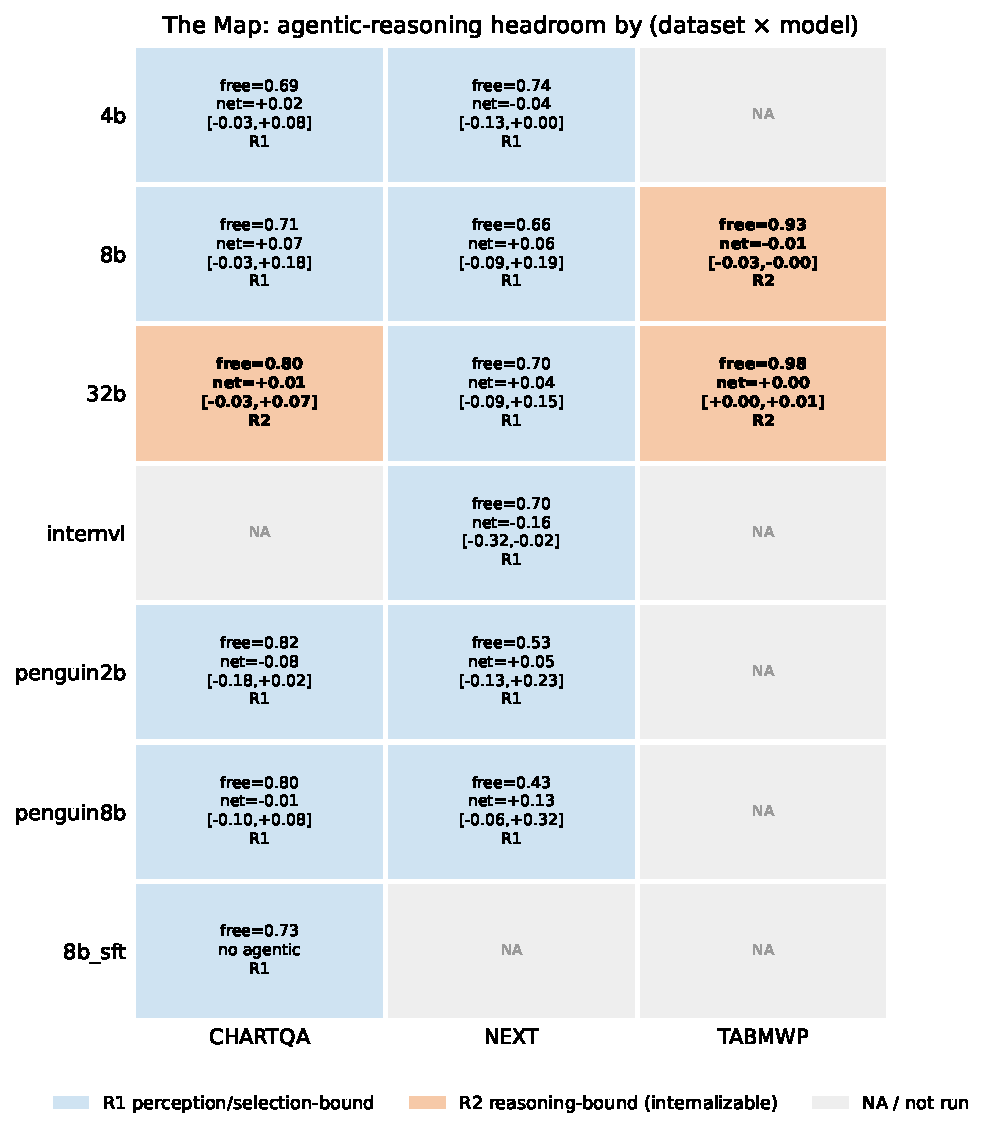
\includegraphics[width=0.6\textwidth]{figures/fig_map.pdf}
  \caption{\textbf{The map.} Variance-gated agentic-reasoning headroom per (dataset $\times$ model).
  Only 32B-on-ChartQA is reasoning-bound (R2); every other cell is perception/selection-bound (R1).}
  \label{fig:map}
\end{figure}

\begin{figure}[t]
  \centering
  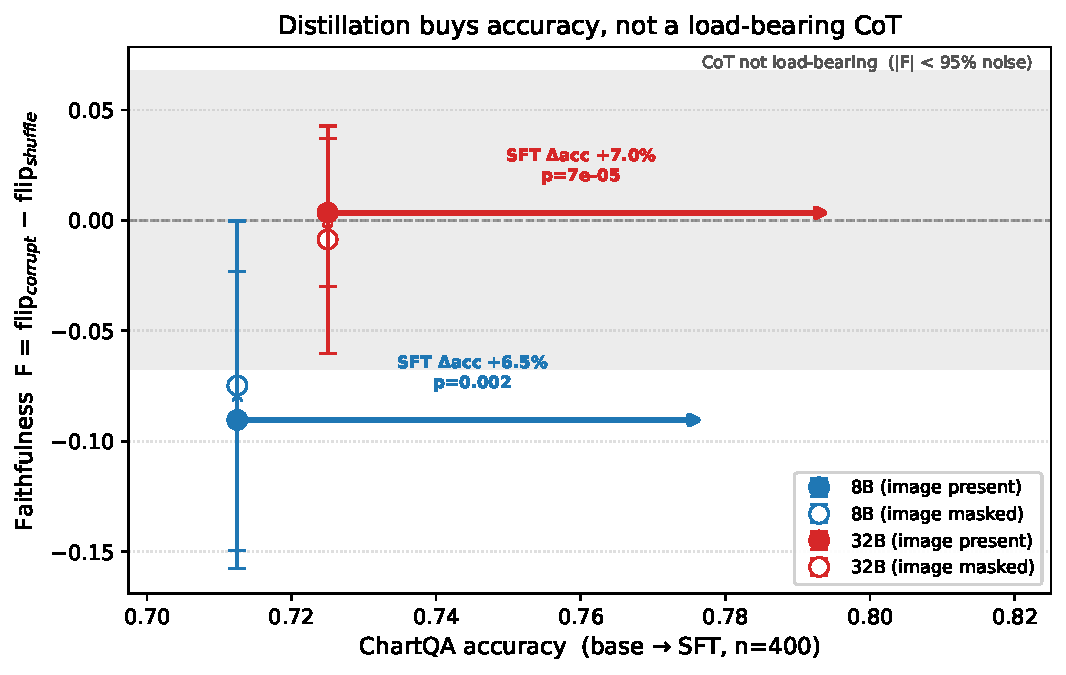
\includegraphics[width=\columnwidth]{figures/fig_decoupling.pdf}
  \caption{\textbf{Accuracy $\perp$ faithfulness.} CoT distillation lifts ChartQA accuracy by
  $+6.5$--$7.0\%$ (McNemar $p\!\le\!.002$; horizontal arrows), yet the internalized CoT stays on the
  $F\!\approx\!0$ band: corrupting a CoT intermediate flips the answer no more than shuffling it.
  A latent chain surfaces only when the image is masked (hollow markers). $F$ is measured on the base;
  error bars are $95\%$ binomial CIs.}
  \label{fig:decoupling}
\end{figure}
